\part{Développement}
\section{Justification des choix techniques}

	\subsection{Bootstrap}

		\href{http://getbootstrap.com/}{Bootstrap} est un framework CSS. Il s'agit d'un ensemble de règles définissant l'apparence de notre page.

		Utiliser Bootstrap nous permet de nous concentrer sur la structure de nos pages, plutôt que de créer nous-même nos styles alors que notre temps est déjà limité.

	\subsection{Git}

		\href{http://git-scm.com/}{Git} est un logiciel de gestion de versions. Il nous permet de gérer différentes versions concurrentes de notre code.

		Git nous a permis de travailler ensemble sur ce projet.

\section{Procédures de tests}
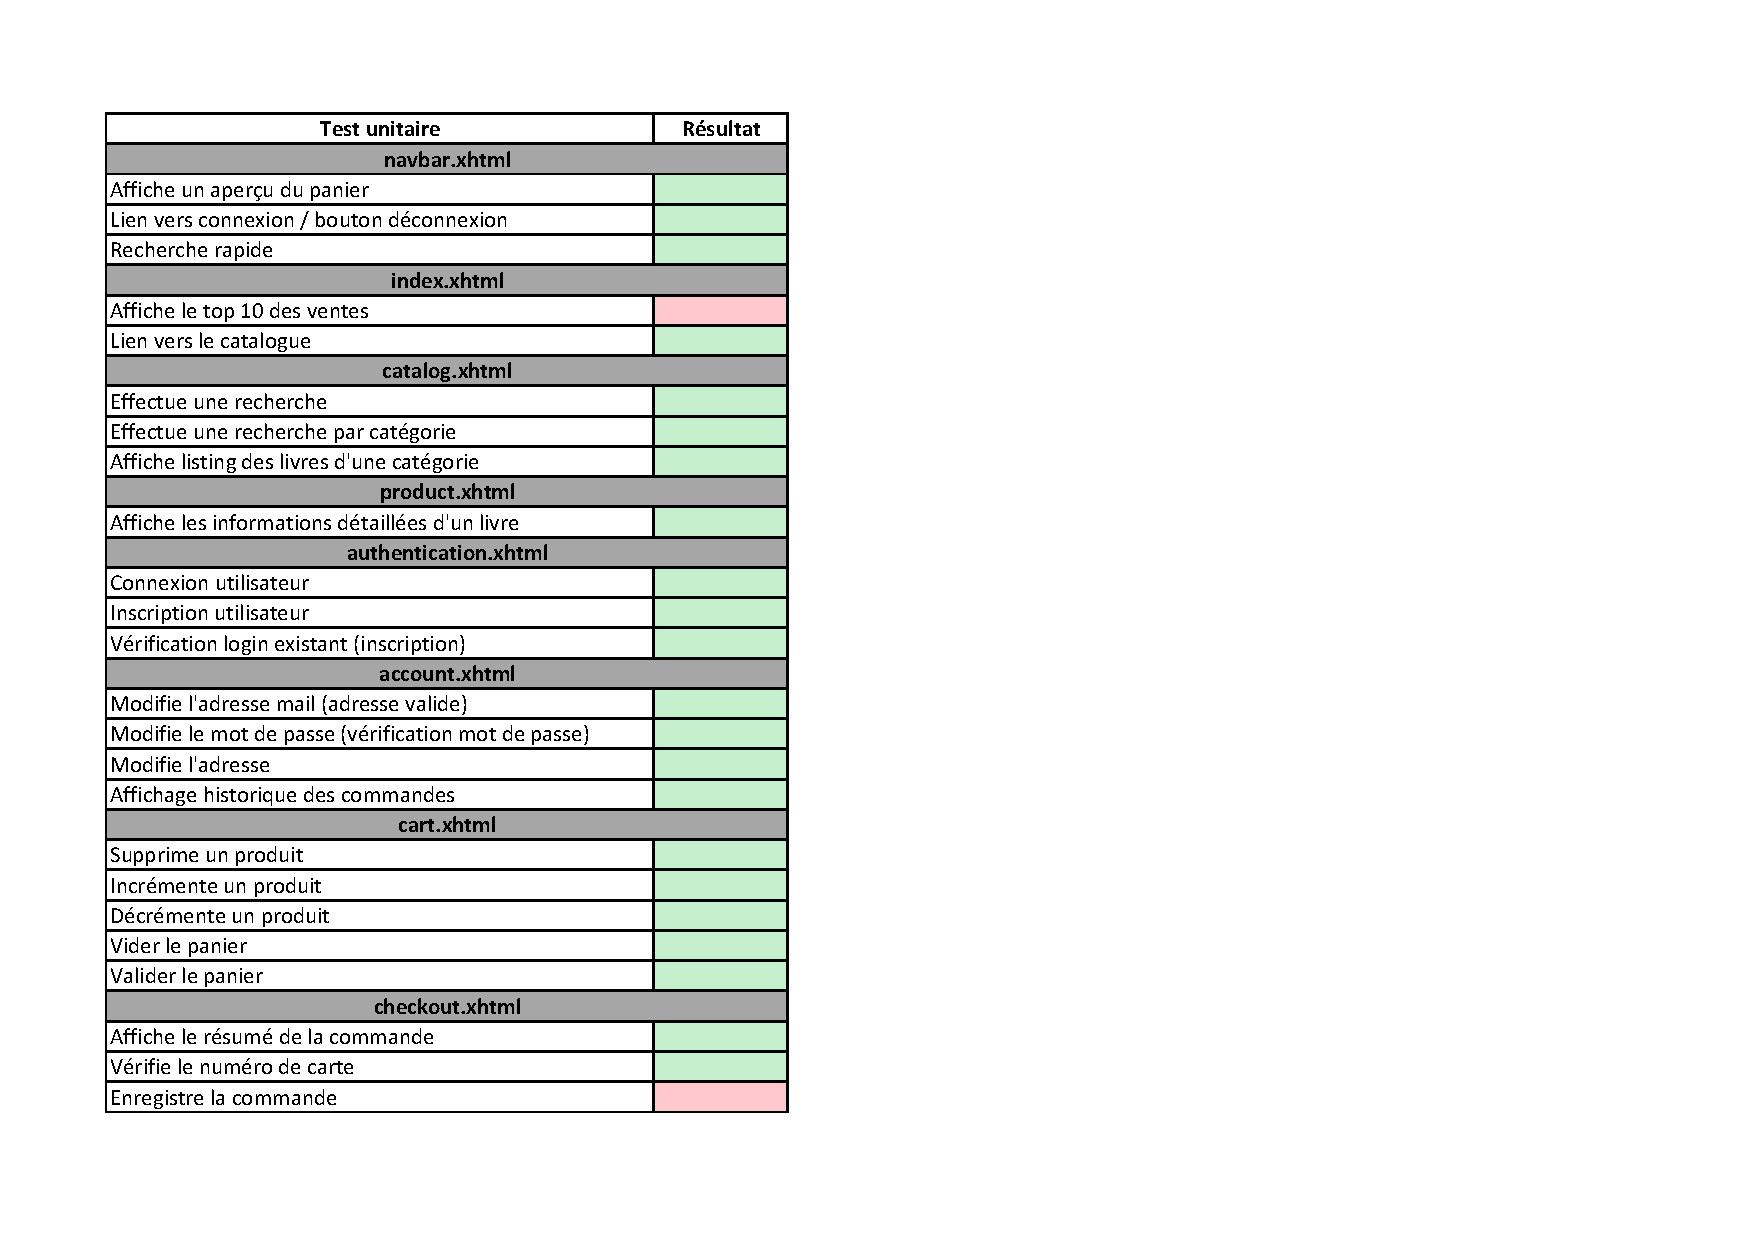
\includepdf[noautoscale=true,offset=150 0]{Res/tests.pdf}
\clearpage
\section{Conception UML}
\subsection{Diagramme d'activité}
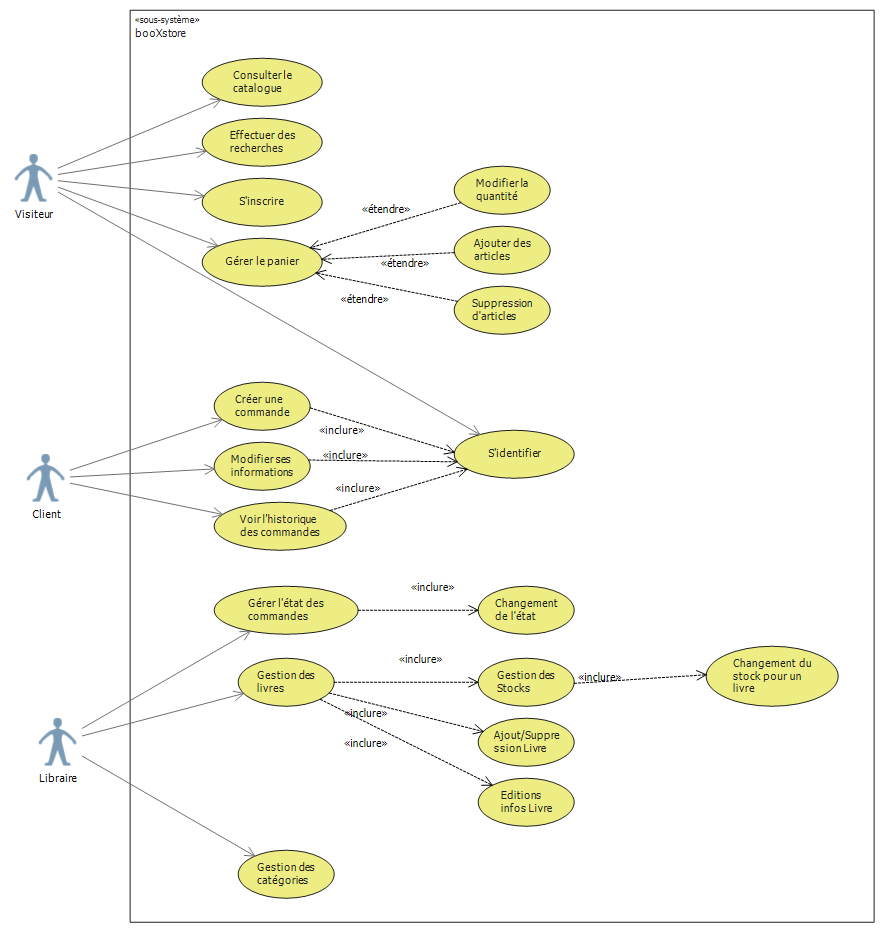
\includegraphics[scale=0.4]{Res/useCase.png}
Le diagramme des cas d'utilisation à été crée pour nous fournir une représentation visuelle
des relations entre les différentes fonctionnalités de l'application. Ainsi que de nous fournir un récapitulatif de ces dernières.\\

Nous voyons ici que l'utilisateur lambda à accès à la consultation du catalogue, aux fonctions de recherche, à l'inscription, à la gestion de son panier(comprenant la modification de la quantité des articles contenus, l'ajout/ l asuppression d'articles)

L'utilisateur peut également décider de se connecter/s'inscrire pour devenir client, ce qui lui donnera accès aux fonctions de création de commande, de modification des informations personnelles ainsi qu'a celles d'affchage de l'historique des commandes
\clearpage
\subsection{Diagramme d'activité}
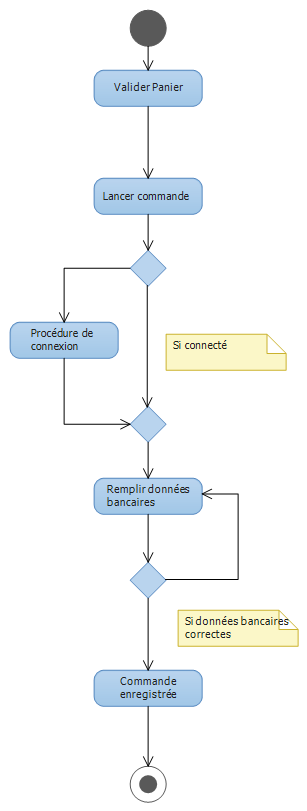
\includegraphics[scale=0.5]{Res/activityCommande.png}\\
Le diagramme d'activité récapitule l'intégralités des actions à effectuer par l'utilisateur afin de créer une nouvelle commande.

Une fois le panier rempli, l'utilisateur va demander à le valider, cette validation va lancer la création de la commande. Si l'utilisateur n'est pas connecté, l'application va demander à l'utilisateur de se connecter.
Si l'utilisateur était conecté, alors on passe à la phase de remplissage des données bancaires. Une fois validée, les données sont vérifiées. Le client devra ressaisir des coordonnées bancaire jusqu'a ce qu'elles soinet valides.
Une fois cette vérification effectuée, la commande est enregistrée.
\clearpage
\subsection{Diagrammes de séquences}
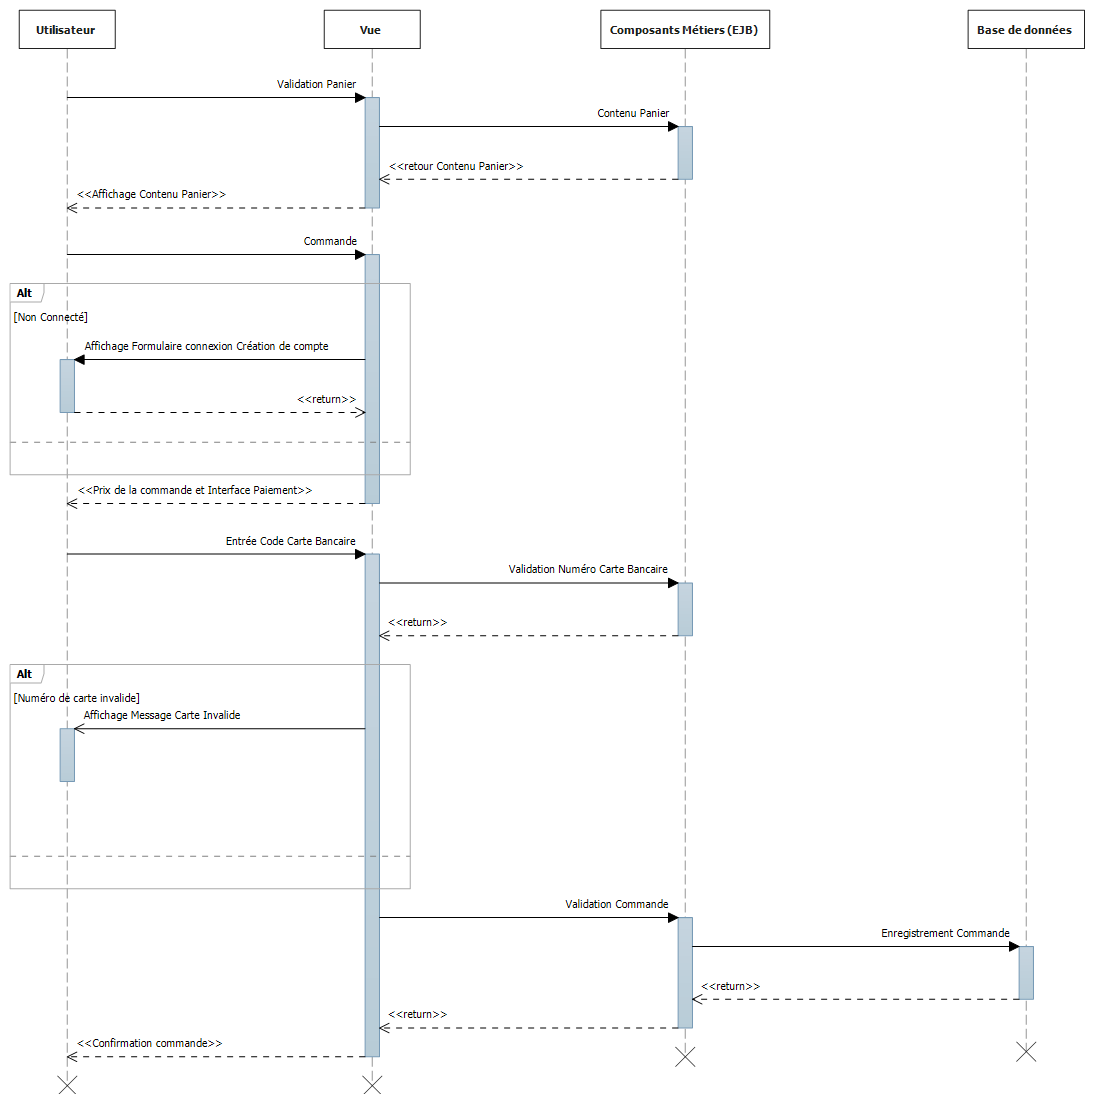
\includegraphics[scale=0.39]{Res/sequenceDiagramOrder.png}
Ce diagramme de séquence décrit les intéractions entre les différentes couches de l'applications nécessaires pour la création d'une commande.
Une fois la validation du panier effectuée par le client, le signal de validation est envoyé à la vue. vue qui demande le contenu du panier au composant métier dédié.
Le client valide alors sa commande. Si il n'est pas connecté la Vue lui affiche alors le formulaire de connexion/inscription. Une fois la connexion faite la vu demande à l'utilisateur de rentrer
ses informations bancaires. Si le numéro entré est invalide, on affiche un message d'erreur  à l'utilisateur et on redemande la saisie.
Si le numéro est validé, on envoie un message de validation de  la commande au composant métier qui va enregistrer la commande en base de données.
Une fois la commande enregistrée, la base renverra une confirmation au composant métier qui renverra lui même une confirmation à la vue qui informera l'utilisateur de la réussite de l'opération.
\clearpage
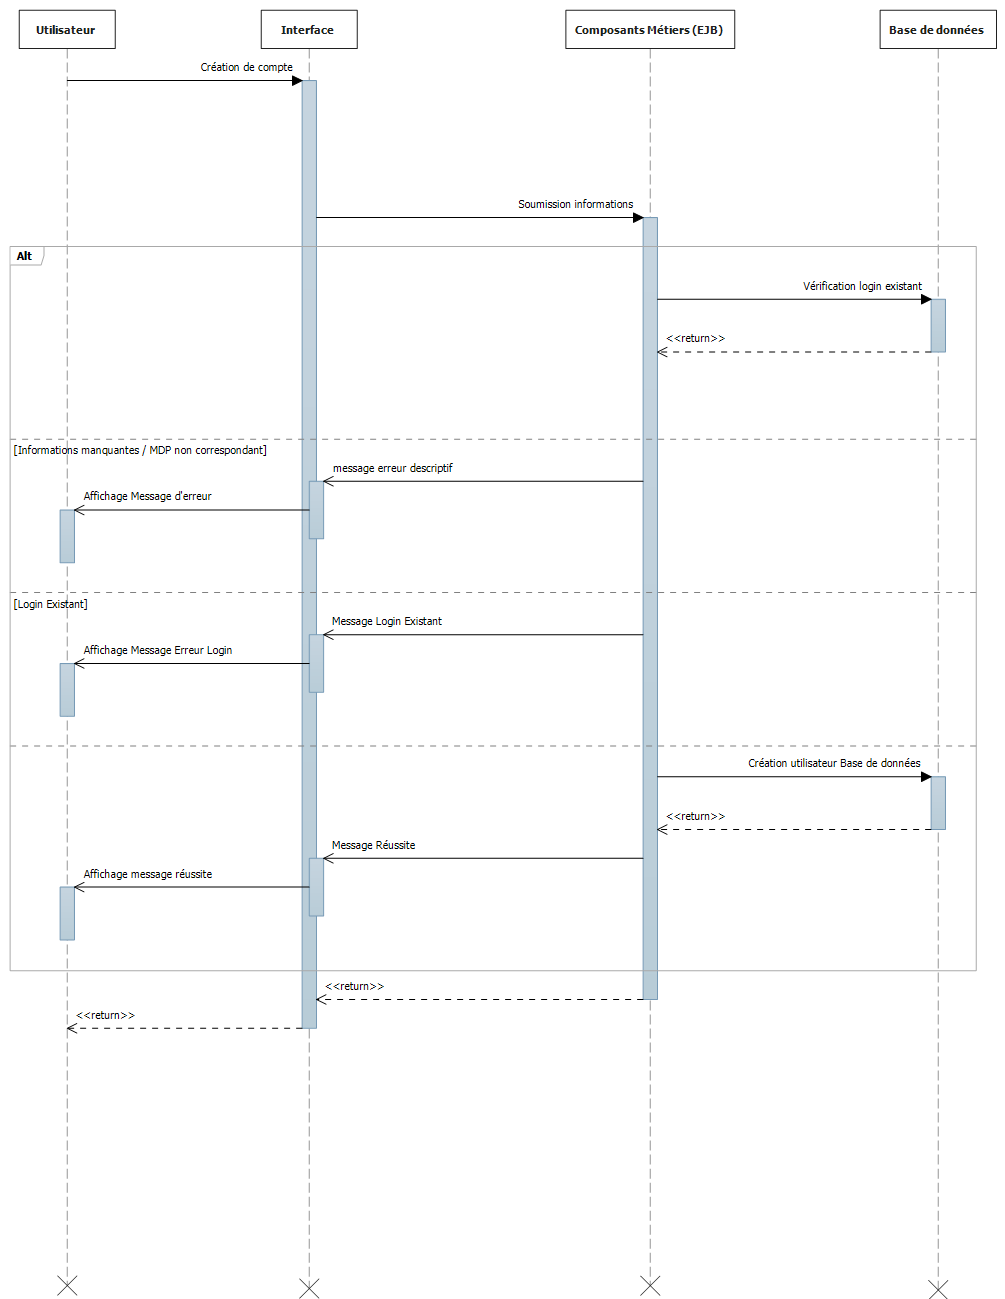
\includegraphics[scale=0.37]{Res/accountCreationSequence.png}
Ce diagramme de séquence décrit les intéractions entre les différeentes couches de l'application nécessaires pour la création d'un compte utilisateur.
Une fois que l'utilisateur à inscrit ses donnéees dans le formulaire d'inscription, l'interface soumet les informations au comosant métier qui va vérifier en base si le login existe déjà.
Si il existe, le composant métier renverra un message à la vue qui affichera un message d'erreur à l'utilisateur qui devra choisir un login différend.
Si une autre erreur est détectée, l'interface l'affichera de la même manière.
Si les informations sont correctes, le composant métier crééra l'utilisateur en base et en inofrmera la vue qui à son tour en informera l'utilisateur.
\clearpage
\subsection{Diagramme de composants}
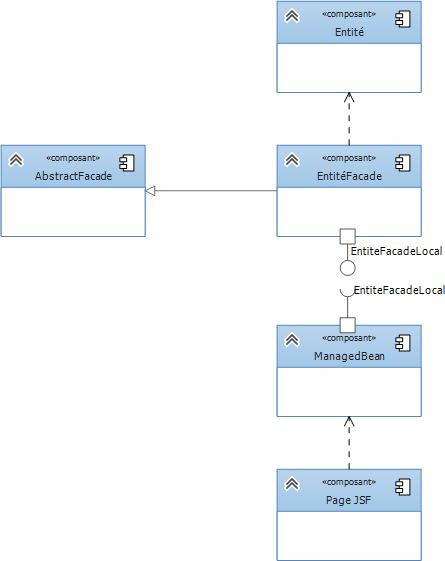
\includegraphics[scale=0.5]{Res/diagrammeComposants.png}\\
Le diagramme de composants à été écrit pour pouvoir généraliser le diagramme de classe qui, Java EE oblige, est très imposant.
Ce diagramme décrit donc que les SessionBeans sont nommés selon le nom de l'entité qu'ils sont censés gérer. Qu'ils implémentent une interface locale et héritent de la classe abstraite AbstractFacade qui gère les opérations CRUD communes.
Les ManagedBeans intancient les SessionBeans correspondants aux interfaces locales et permettent aux pages JSF d'accéder aux informations stockées en base de données.
\subsection{Diagramme de classe}
\clearpage
\begin{figure}[h!]
\includepdf{Res/classDiagram.pdf}
\end{figure}
\clearpage
Au vu de la taille du diagramme, il se peut que celui-ci ne soit pas lisible sur une feuille A4, voici un lien pour le télécharger à part : \href{http://goo.gl/D9HGij}{http://goo.gl/D9HGij}
\section{Points forts et points faibles de notre implémentation}

	\subsection{Points forts}
	\begin{itemize}
		\item \textbf{La navbar :} Elle permet une utilisation rapide de la recherche de livre au lieu de voyager au travers des catégories afin d'avoir le livre qui nous convient le plus. La connexion/inscription de l'utilisateur est aussi présente sur celle-ci. Et pour conclure sur cette navbar, le panier affiche le pris et le nombre d'article de la commande en cours de l'utilisateur. Il lui reste ensuite qu'à cliquer dessus pour valider sa commande et passer au payement.

		\item \textbf{Bootstrap :} Les pages crées avec ce style, permet d'avoir des pages intuitives pour les utilisateurs du store. L'esthétique/L'intuitivité du site est également important pour que l'utilisateur trouve ces repères rapidement et puisse ainsi revenir s'il trouve que le site lui plait.

		\item Nos pages du store s'adapte également au fenêtre qu'on lui impose si elle est petite la navbar s'adapte à celle-ci et devient un bouton ou l'on clique dessus pour afficher le reste du menu.
	\end{itemize}


	\subsection{Point faible}
	\begin{itemize}
		\item Le temps de chargement de la page de gestions des libraires est trop longue à s'ouvrir/charger vu le nombre de données qui doit être afficher sur celle-ci. Cette page (management.xhmtl) peut-être optimisée pour devenir plusieurs pages au lieu de faire des onglets. En gros, un onglet devient une page.
	\end{itemize}
